\documentclass[10.5pt]{config}
% 本实验报告采用 署名-相同方式共享 4.0 国际许可协议 (CC BY-SA 4.0)

\major{电子科学与技术}
\name{郑智瑄}
\partner{} % 签名栏
% \title{}
\stuid{3230103913}
\date{\today}
\lab{西2-310}
\course{信号与系统}
\instructor{陈晓明}
\grades{}
\expname{Lab01} % 实验名字
\exptype{Matlab仿真} % 实验类型

\begin{document}

% \maketitlepage % 封面
% \maketoc % 目录
\makeheader % 首页头部

\section{Problem1}
\subsection{Question}
\begin{figure}[!htbp]
  \centering
  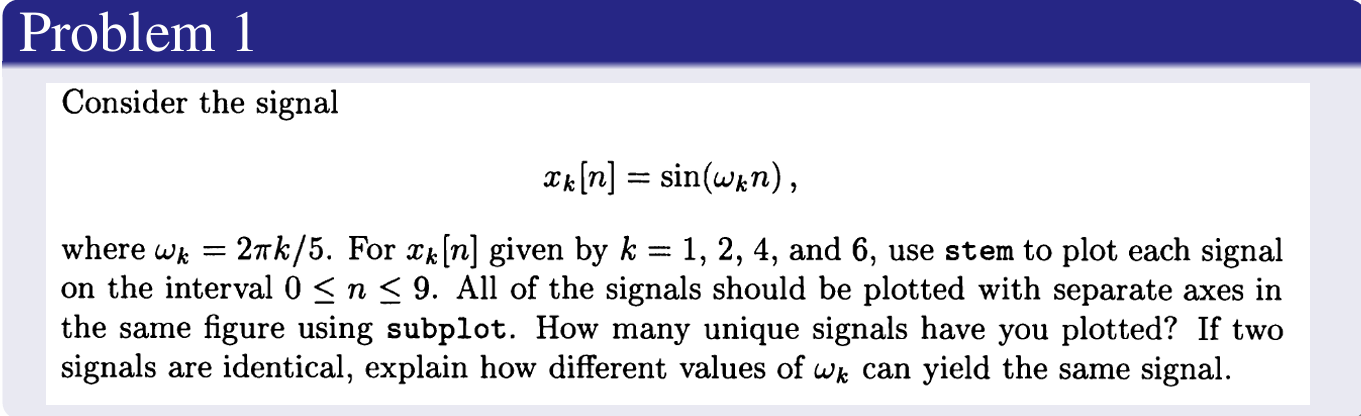
\includegraphics[width=1\linewidth]{figures/Q1.jpg} % 数字表示放缩比例
  \caption{Problem1} % 图片标题
  \label{fig:Problem1} % 图片tag，用于交叉引用
\end{figure}
\subsection{Code}
\begin{lstlisting}[language=matlab, caption=Problem1 Code]
  %Lab1 P1

  clc;clear;
  
  n = 0:9;
  k_values = [1, 2, 4, 6];
  
  figure;
  
  for i = 1:length(k_values)
      k = k_values(i);
      wk = 2 * pi * k / 5;
      Tk = sin(wk * n);
      
      subplot(4, 1, i);
      stem(n, Tk, 'filled');
      title(['k = ', num2str(k)]);
      xlabel('n');
      ylabel('T_k[n]');
      grid on;
  end
  
  sgtitle('Signals T_k[n] = sin(w_k n) for different k values');
  
\end{lstlisting}

\subsection{Figure}
\begin{figure}[!htbp]
  \centering
  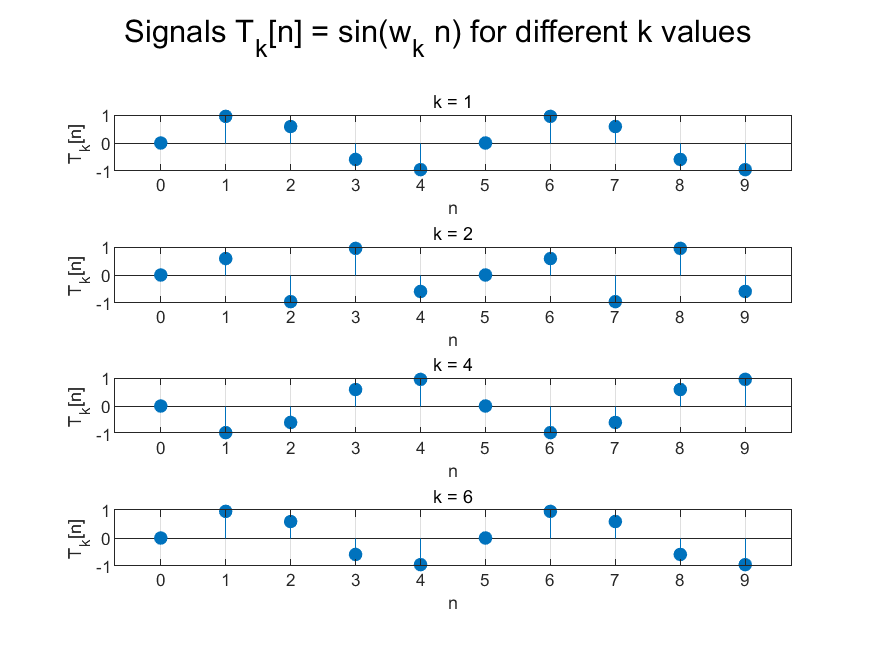
\includegraphics[width=0.9\linewidth]{figures/P1.jpg} % 数字表示放缩比例
  \caption{Problem1 Result} % 图片标题
  \label{fig:Problem2 Result} % 图片tag，用于交叉引用
\end{figure}


\subsection{Answer}
There are three unique signals

When different $\omega$ values differ by integer multiples of $2\pi$, the corresponding discrete-time signals will be the same.
\clearpage
\section{Problem2}
\subsection{Question}
\begin{figure}[!htbp]
  \centering
  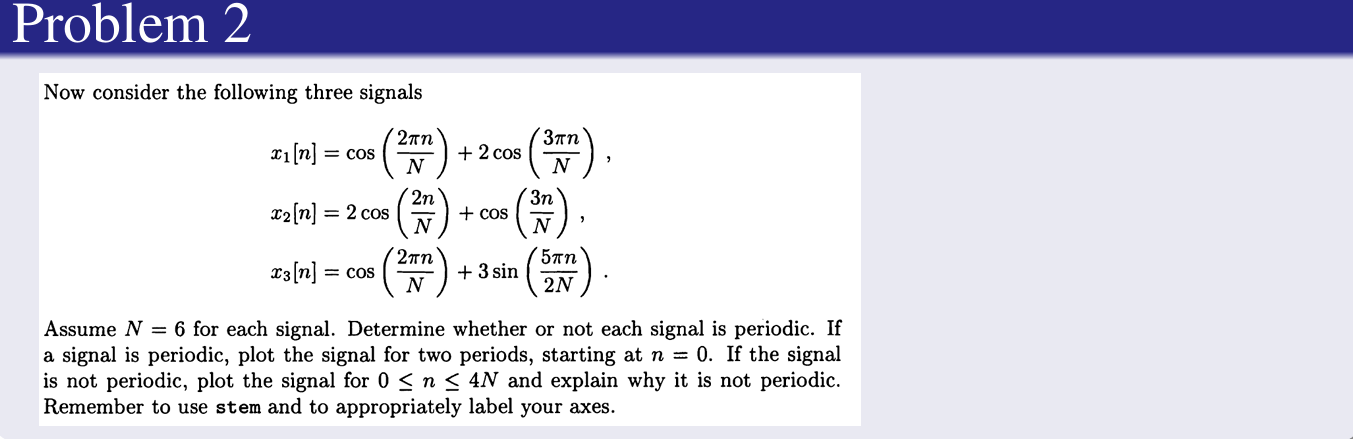
\includegraphics[width=1\linewidth]{figures/Q2.jpg} % 数字表示放缩比例
  \caption{Problem2} % 图片标题
  \label{fig:Problem2} % 图片tag，用于交叉引用
\end{figure}
\subsection{Code}
\begin{lstlisting}[language=matlab, caption=Problem2 Code]
  %Lab1 P2

  clc;clear;

  N = 6;
  n_periodic_x1 = 0:24;
  n_non_periodic = 0:4*N;
  n_periodic_x3 = 0:48;

  x1 = cos(2*pi*n_periodic_x1/N) + 2*cos(3*pi*n_periodic_x1/N);
  x2 = 2*cos(2*n_non_periodic/N) + cos(3*n_non_periodic/N);
  x3 = cos(2*pi*n_periodic_x3/N) + 3*sin(5*pi*n_periodic_x3/2/N);

  figure;

  subplot(3, 1, 1);
  stem(n_periodic_x1, x1, 'filled');
  title('x_1[n] = cos(2\pi n/N) + 2cos(3\pi n/N) :period is 2N=12');
  xlabel('n');
  ylabel('x_1[n]');
  grid on;

  subplot(3, 1, 2);
  stem(n_non_periodic, x2, 'filled');
  title('x_2[n] = 2cos(2n/N) + cos(3n/N) :Not periodic');
  xlabel('n');
  ylabel('x_2[n]');
  grid on;
  
  subplot(3, 1, 3);
  stem(n_periodic_x3, x3, 'filled');
  title('x_3[n] = cos(2\pi n/N) + 3sin(5\pi n/2N) :period is 4N=24');
  xlabel('n');
  ylabel('x_3[n]');
  grid on;

  sgtitle('Periodicity Analysis of Signals');

    
\end{lstlisting}

\subsection{Figure}
\begin{figure}[!htbp]
  \centering
  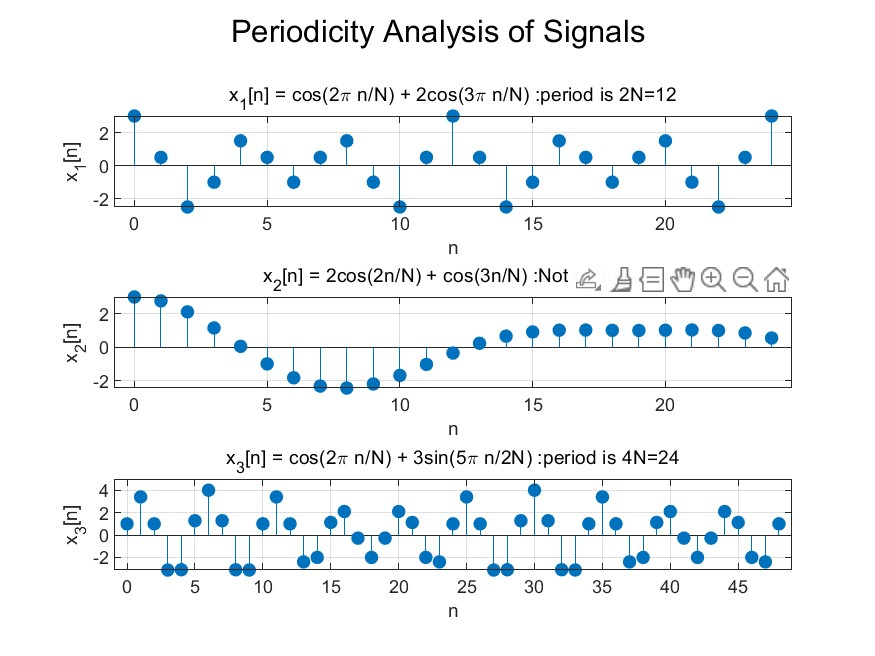
\includegraphics[width=0.75\linewidth]{figures/P2.jpg} % 数字表示放缩比例
  \caption{Problem2 Result} % 图片标题
  \label{fig:Problem2 Result} % 图片tag，用于交叉引用
\end{figure}
\subsection{Answer}
$x_1[n]$: $T=2N=12$

$x_2[n]$: $T1=N\pi$ and $T2=\frac{2N}{3}\pi$;$T=2N*\pi$,which is irrational,so $x_2[n]$ isn't periodic

$x_3[n]$: $T=4N=24$
\clearpage
\section{Problem3}
\subsection{Question}
\begin{figure}[!htbp]
  \centering
  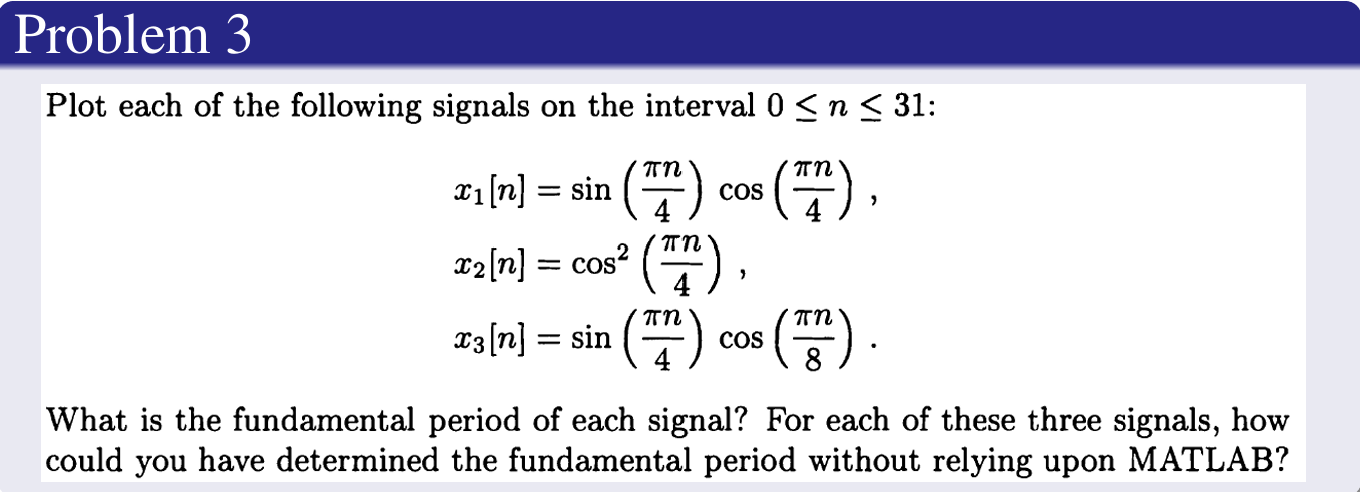
\includegraphics[width=1\linewidth]{figures/Q3.jpg} % 数字表示放缩比例
  \caption{Problem3} % 图片标题
  \label{fig:Problem3} % 图片tag，用于交叉引用
\end{figure}
\subsection{Code}
\begin{lstlisting}[language=matlab, caption=Problem3 Code]
  %Lab1 P3

  clc;clear;

  n = 0:31;

  x1 = sin(pi*n/4) .* cos(pi*n/4);
  x2 = cos(pi*n/4).^2;
  x3 = sin(pi*n/4) .* cos(pi*n/8);

  figure;

  subplot(3,1,1);
  stem(n, x1,'filled');
  title('Signal x1[n] = sin(\pi n / 4) cos(\pi n / 4)');
  xlabel('n');
  ylabel('x1[n]');

  subplot(3,1,2);
  stem(n, x2,"filled");
  title('Signal x2[n] = cos^2(\pi n / 4)');
  xlabel('n');
  ylabel('x2[n]');

  subplot(3,1,3);
  stem(n, x3,"filled");
  title('Signal x3[n] = sin(\pi n / 4) cos(\pi n / 8)');
  xlabel('n');
  ylabel('x3[n]');
\end{lstlisting}

\subsection{Figure}
\begin{figure}[!htbp]
  \centering
  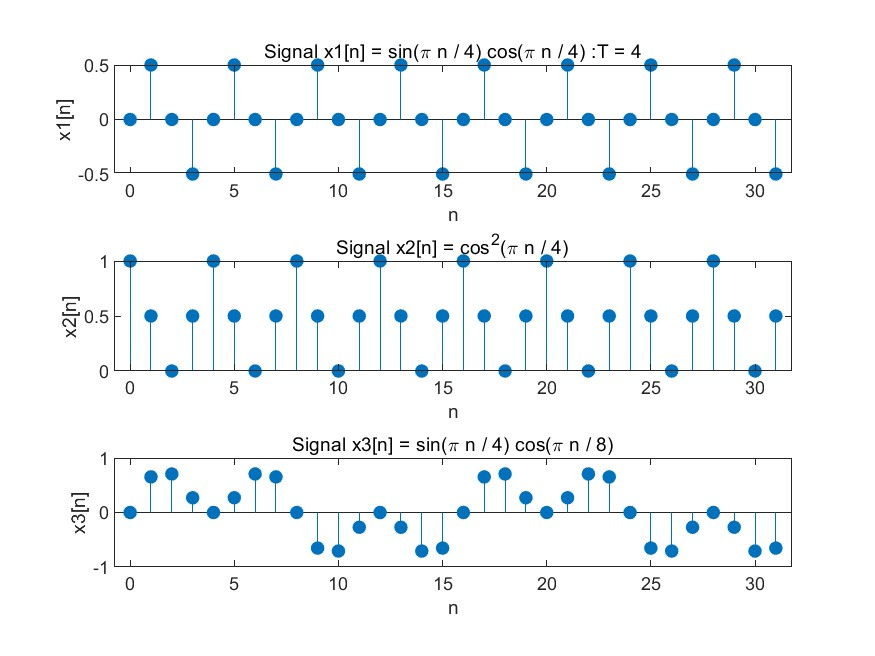
\includegraphics[width=0.9\linewidth]{figures/P3.jpg} % 数字表示放缩比例
  \caption{Problem3 Result} % 图片标题
  \label{fig:Problem3 Result} % 图片tag，用于交叉引用
\end{figure}
\subsection{Answer}
$$x_1 = \frac{1}{2}sin(\frac{\pi n}{2}) \Rightarrow x_1[n]:T=4$$
$$x_2 = \frac{1}{2}[1+cos(\frac{\pi n}{2})] \Rightarrow x_2[n]:T=4$$
$$x_3 = \frac{1}{2}[sin(\frac{3\pi n}{8}) + sin(\frac{\pi n}{8})] \Rightarrow x_3[n]:T = 16$$
\clearpage
\section{Problem4}
\subsection{Question}
\begin{figure}[!htbp]
  \centering
  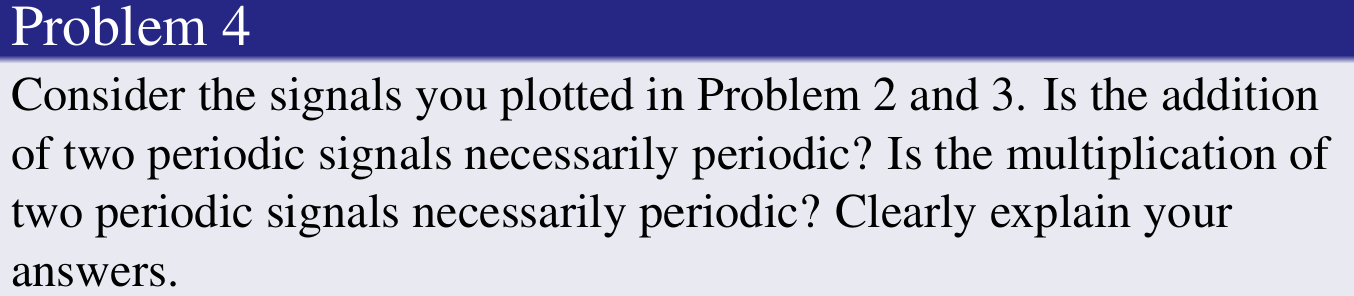
\includegraphics[width=1\linewidth]{figures/Q4.jpg} % 数字表示放缩比例
  \caption{Problem4} % 图片标题
  \label{fig:Problem4} % 图片tag，用于交叉引用
\end{figure}
\subsection{Answer}
\subsubsection{The addtion of two periodic signals isn't necessarily periodic
}
for continuous signal:
$$ f(t) = cos2\pi t+cost$$
$$f(t+T) = cos(2\pi t+2\pi T)+cos(t+T)$$
$$T = k\ and\ T = 2k\pi , k \in N $$

it is contradictory, so isn't necessarily periodic

for discrete signal,it is periodic
\subsubsection{The multiplication of two periodic signals isn't necessarily periodic
}
for continuous signal:
$$f(t) = cos\frac{2\pi+1}{2}t \* cos\frac{2\pi -1}{2}t =\frac{1}{2} (cos2\pi t+cost)$$

which is not periodic, so isn't necessarily periodic
% $$ f(t) = cos2\pi t \* cost=\frac{1}{2} [cos(2\pi +1)t+cos(2\pi -1)t]$$
% $$f(t+T) = \frac{1}{2} \{ cos[(2\pi+1) t+(2\pi +1)T] + cos[(2\pi-1) t+(2\pi -1)T]\}$$
% $$T = k\ and\ T = 2k\pi , k \in N $$
% $$is \ contradictory$$

for discrete signal,it is periodic
\clearpage
\section{Problem5}
\subsection{Question}
\begin{figure}[!htbp]
  \centering
  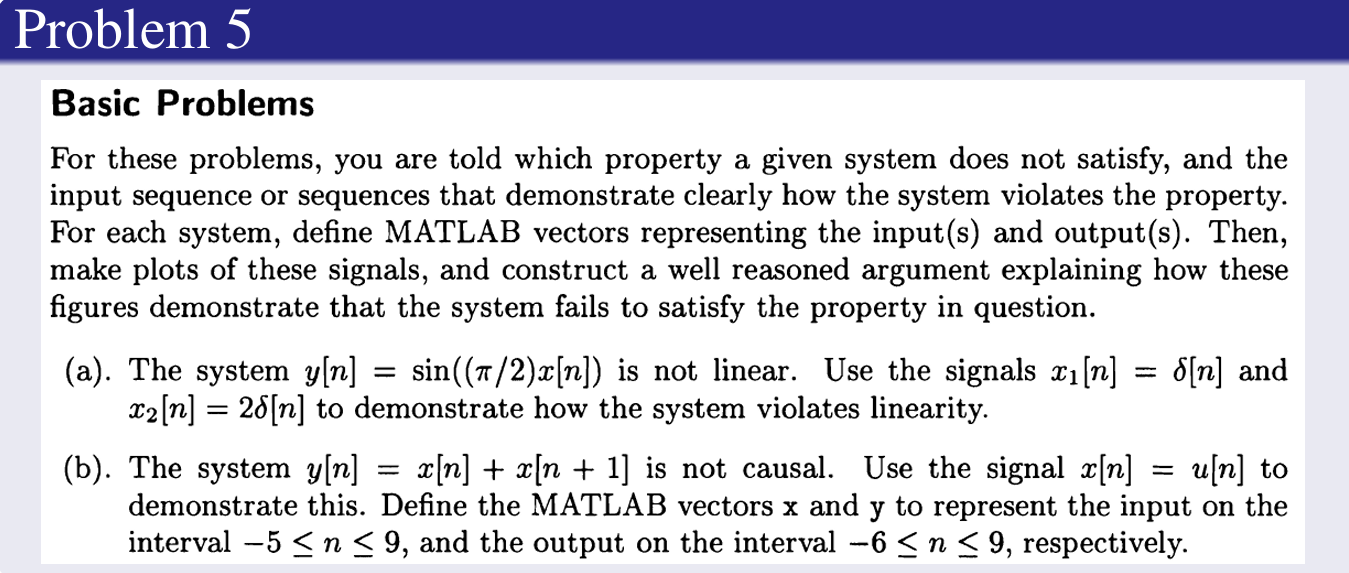
\includegraphics[width=1\linewidth]{figures/Q5.jpg} % 数字表示放缩比例
  \caption{Problem5} % 图片标题
  \label{fig:Problem5} % 图片tag，用于交叉引用
\end{figure}
\subsection{Code}
\begin{lstlisting}[language=matlab, caption=Problem5a Code]
  %Lab1 P5a

  clc;clear;
  n = -5:5;
  delta = (n == 0);
  x1 = delta;
  x2 = 2*delta;
  y1 = sin(pi/2 * x1);
  y2 = sin(pi/2 * x2);

  figure;

  subplot(2,1,1);
  stem(n, y1,"filled");
  title('y1[n] = sin(\pi/2 * x1[n])');
  xlabel('n');
  ylabel('y1[n]');

  subplot(2,1,2);
  stem(n, y2,"filled");
  title('y2[n] = sin(\pi/2 * x2[n])');
  xlabel('n');
  ylabel('y2[n]');
  sgtitle('Analysis of Signals Property :y_2[0]!=2y_1[0],not linear');
\end{lstlisting}

\begin{lstlisting}[language=matlab, caption=Problem5b Code]
  %Lab1 P5 b

  clc;clear;
  n = -5:9;
  u = @(n) double(n >= 0);
  x = u(n);
  y = u(n)+u(n+1);

  figure;
  subplot(2,1,1);
  stem(n, x,"filled");
  title('Input x[n] = u[n]');
  xlabel('n');
  ylabel('x[n]');

  subplot(2,1,2);
  stem(n, y,"filled");
  title('Output y[n] = x[n] + x[n+1]');
  xlabel('n');
  ylabel('y[n]');
\end{lstlisting}
\subsection{Figure}
\begin{figure}[!htbp]
  \centering
  \begin{minipage}[b]{0.5\linewidth}
      \centering
      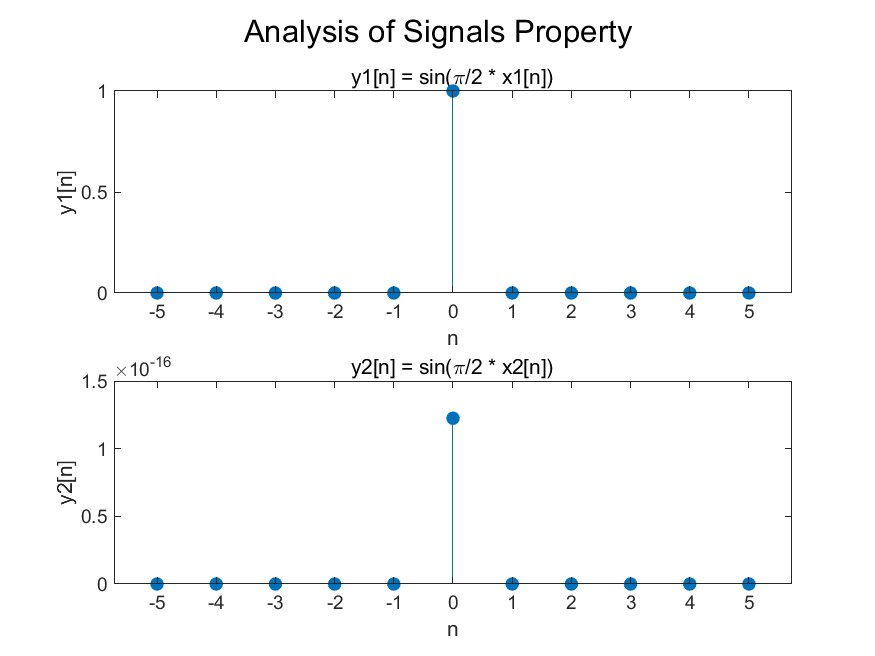
\includegraphics[width=0.9\textwidth]{figures/P5a.jpg}
      \caption{Problem5a Result}
  \end{minipage}%
  \begin{minipage}[b]{0.5\linewidth}
      \centering
      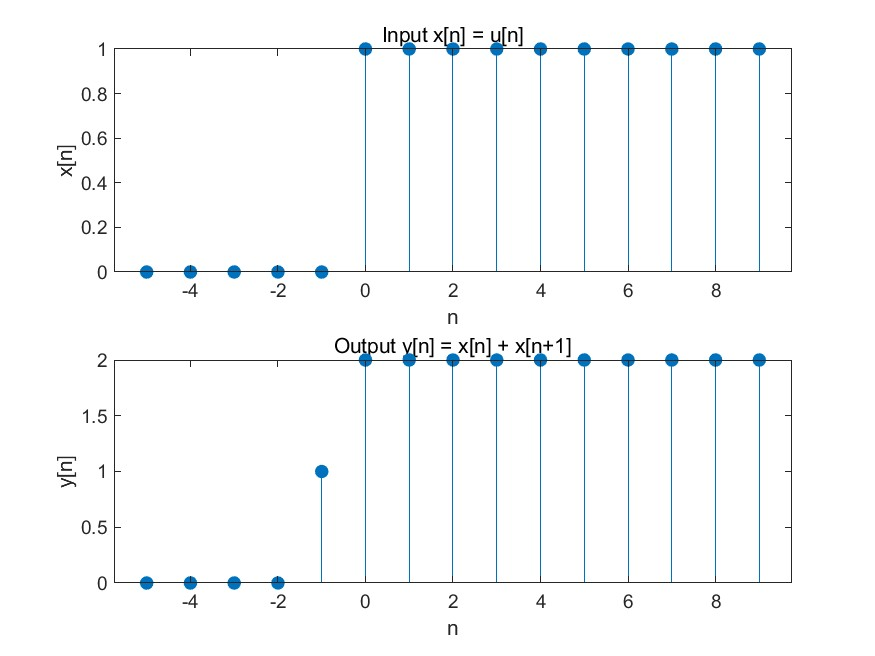
\includegraphics[width=0.9\textwidth]{figures/P5b.jpg}
      \caption{Problem5b Result}
  \end{minipage}
\end{figure}
\subsection{Answer}
P5a:Non-Linear Verification:
$$y_2[n] \neq 2y_1[n],$$

P5b:Non-Causality Verification: The system uses x[n+1] (future input) to compute y[n]
\clearpage
\section{Problem6}
\subsection{Question}
\begin{figure}[!htbp]
  \centering
  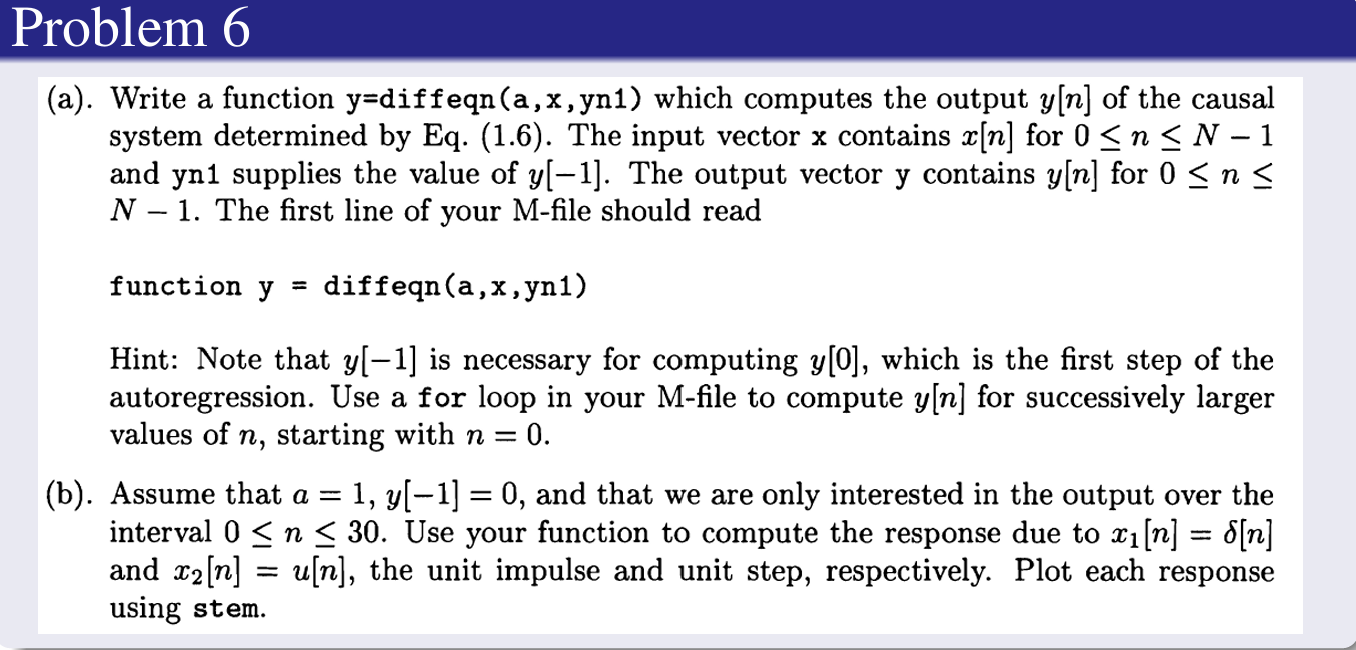
\includegraphics[width=1\linewidth]{figures/Q6.jpg} % 数字表示放缩比例
  \caption{Problem6} % 图片标题
  \label{fig:Problem6} % 图片tag，用于交叉引用
\end{figure}
\subsection{Code}
\begin{lstlisting}[language=matlab, caption=Problem6 Code]
  %Lab1 P6

  function y = diffeqn(a, x, yn1)
      N = length(x);
      y = zeros(1, N);
      y(1) = a * yn1 + x(1);

      for i = 2:N
          y(i) = a * y(i-1) + x(i);
      end
  end

  n = 0:30;
  x1 = (n == 0);
  x2 = (n >= 0);
  yn1 = 0;
  a = 1;
  y1 = diffeqn(a, x1, yn1);
  y2 = diffeqn(a, x2, yn1);

  figure;
  subplot(2,1,1);
  stem(n, y1,"filled");
  title('Response to x1[n] = \delta[n]');
  xlabel('n');
  ylabel('y1[n]');

  subplot(2,1,2);
  stem(n, y2,"filled");
  title('Response to x2[n] = u[n]');
  xlabel('n');
  ylabel('y2[n]');
\end{lstlisting}

\subsection{Figure}
\begin{figure}[!htbp]
  \centering
  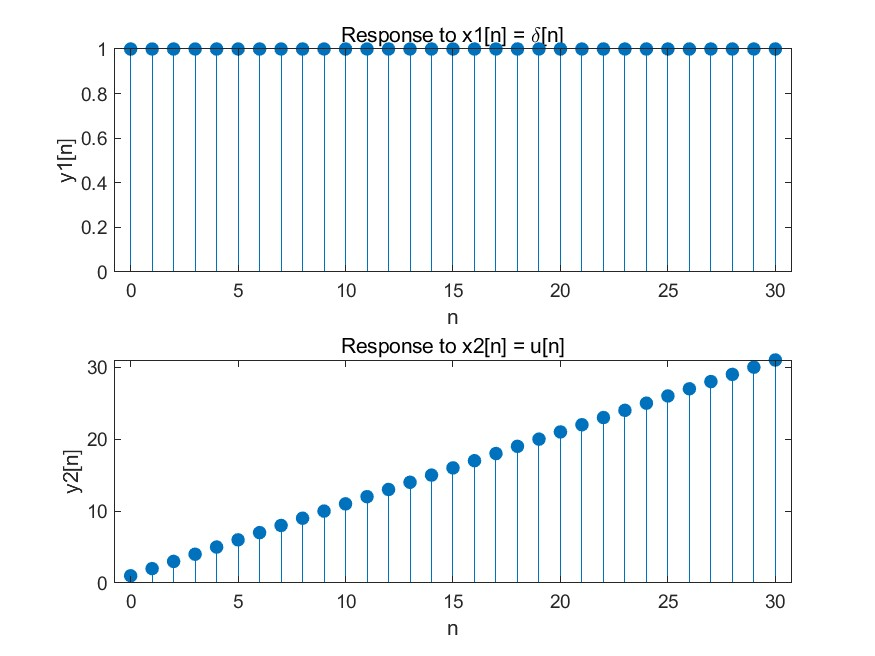
\includegraphics[width=1\linewidth]{figures/P6.jpg} % 数字表示放缩比例
  \caption{Problem6 Result} % 图片标题
  \label{fig:Problem6 Result} % 图片tag，用于交叉引用
\end{figure}
\clearpage
\section{Problem7}
\subsection{Question}
\begin{figure}[!htbp]
  \centering
  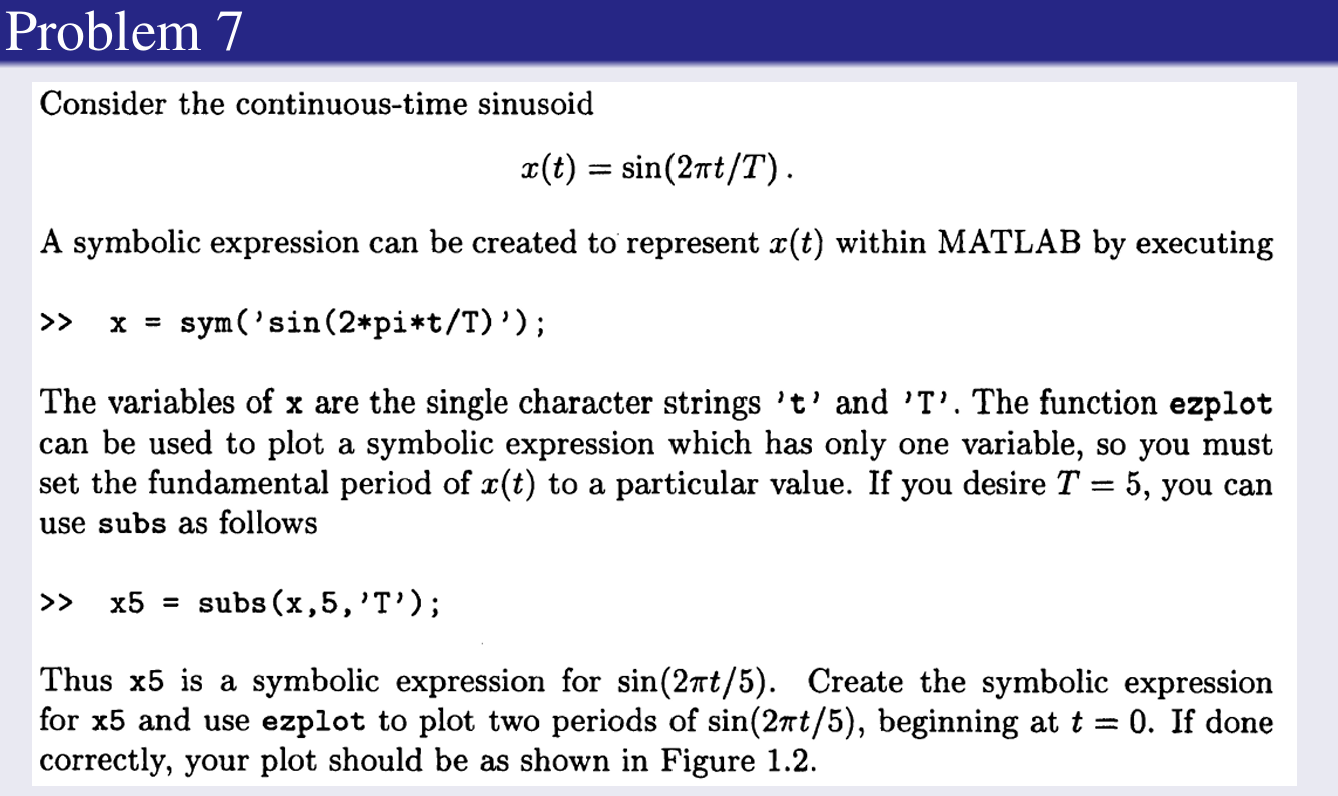
\includegraphics[width=1\linewidth]{figures/Q7.jpg} % 数字表示放缩比例
  \caption{Problem7} % 图片标题
  \label{fig:Problem7} % 图片tag，用于交叉引用
\end{figure}
\subsection{Code}
\begin{lstlisting}[language=matlab, caption=Problem7 Code]
  %Lab1 P7

  syms t T
  x = sin(2*pi*t/T);

  x5 = subs(x, T, 5);

  ezplot(x5, [0, 10])
  grid on
  xlabel('t')
  ylabel('x(t)')
  title('Plot of sin(2\pi t / 5) over two periods')
\end{lstlisting}

\subsection{Figure}
\begin{figure}[!htbp]
  \centering
  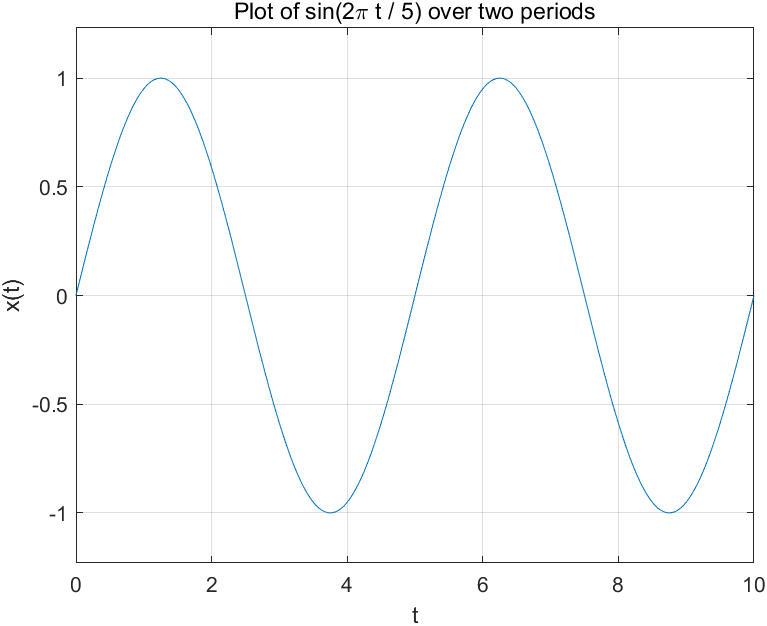
\includegraphics[width=0.75\linewidth]{figures/P7.png} % 数字表示放缩比例
  \caption{Problem7 Result} % 图片标题
  \label{fig:Problem7 Result} % 图片tag，用于交叉引用
\end{figure}
\clearpage
\section{Problem8}
\subsection{Question}
\begin{figure}[!htbp]
  \centering
  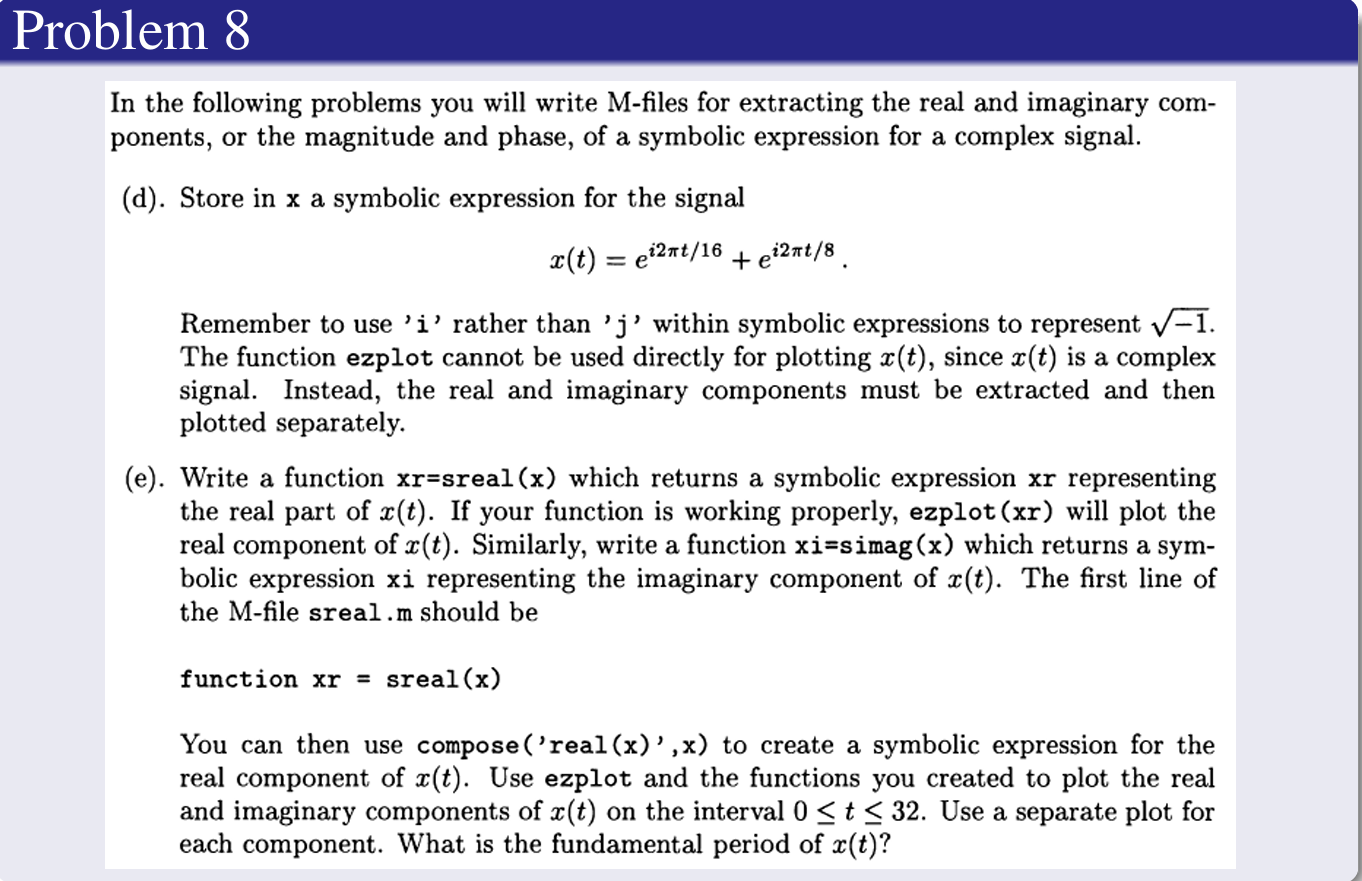
\includegraphics[width=1\linewidth]{figures/Q8.jpg} % 数字表示放缩比例
  \caption{Problem8} % 图片标题
  \label{fig:Problem8} % 图片tag，用于交叉引用
\end{figure}
\subsection{Code}
\begin{lstlisting}[language=matlab, caption=Problem8 Code]
  %Lab1 P8
  
  function xr = sreal(x)
  xr = real(x);
  end

  function xi = simag(x)
    xi = imag(x);
  end

  syms t
  x = exp(1i*2*pi*t/16) + exp(1i*2*pi*t/8);

  xr = sreal(x);
  xi = simag(x);

  figure;
  ezplot(xr, [0, 32])
  grid on
  xlabel('t')
  ylabel('Re\{x(t)\}')
  title('Real Component of x(t)')

  figure;
  ezplot(xi, [0, 32])
  grid on
  xlabel('t')
  ylabel('Im\{x(t)\}')
  title('Imaginary Component of x(t)')

\end{lstlisting}

\subsection{Figure}
\begin{figure}[!htbp]
  \centering
  \begin{minipage}[b]{0.45\linewidth}
      \centering
      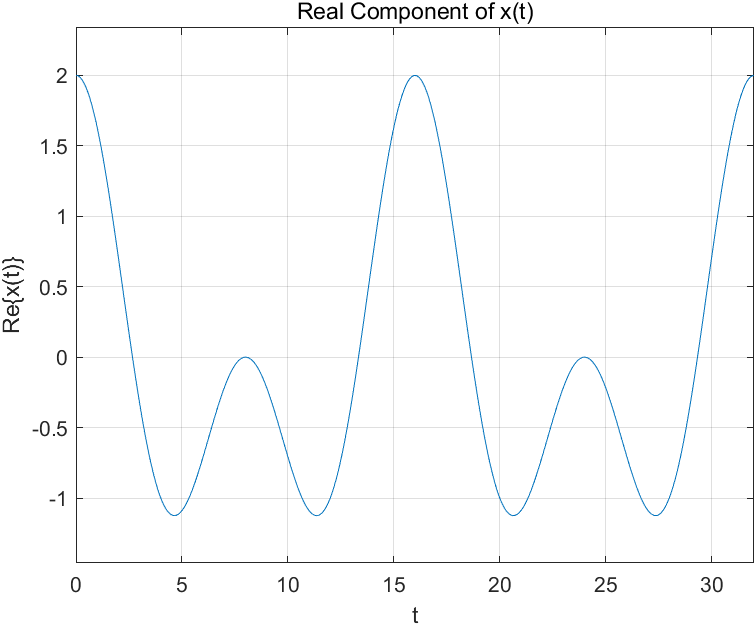
\includegraphics[width=0.9\textwidth]{figures/P8a.png}
      \caption{Problem8a Result}
  \end{minipage}%
  \begin{minipage}[b]{0.45\linewidth}
      \centering
      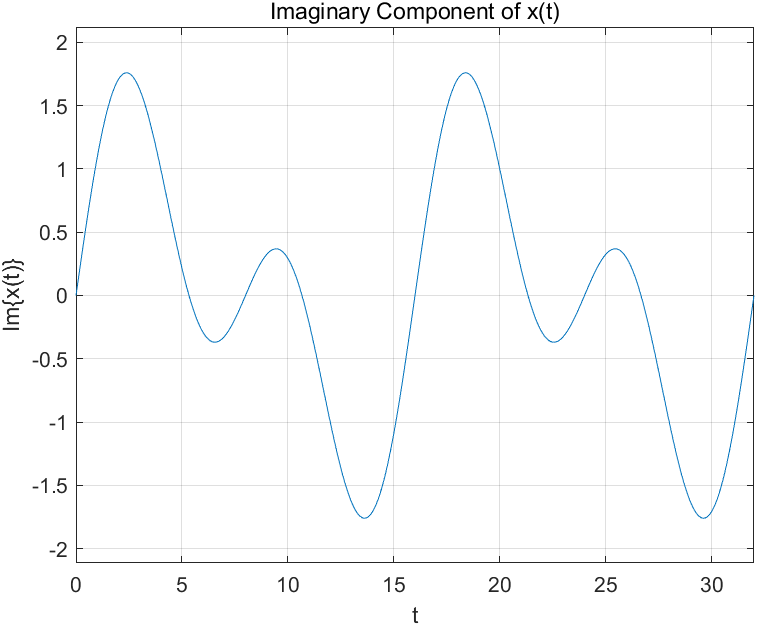
\includegraphics[width=0.9\textwidth]{figures/P8b.png}
      \caption{Problem8b Result}
  \end{minipage}
\end{figure}
\subsection{Answer}
$$The \ fundamental \ period \ of \ x(t) \ is \ 16$$
\end{document}